
% VLDB template version of 2020-08-03 enhances the ACM template, version 1.7.0:
% https://www.acm.org/publications/proceedings-template
% The ACM Latex guide provides further information about the ACM template

\documentclass[sigconf, nonacm]{acmart}

%% The following content must be adapted for the final version
% paper-specific
\newcommand\vldbdoi{XX.XX/XXX.XX}
\newcommand\vldbpages{XXX-XXX}
% issue-specific
\newcommand\vldbvolume{14}
\newcommand\vldbissue{1}
\newcommand\vldbyear{2020}
% should be fine as it is
\newcommand\vldbauthors{\authors}
\newcommand\vldbtitle{\shorttitle} 
% leave empty if no availability url should be set
\newcommand\vldbavailabilityurl{https://github.com/karpen04/RepEng-duckiesProject}
% whether page numbers should be shown or not, use 'plain' for review versions, 'empty' for camera ready
\newcommand\vldbpagestyle{plain} 

\begin{document}
\title{"Duckies" Reproduction Package Project}

%%
%% The "author" command and its associated commands are used to define the authors and their affiliations.
\author{Oleksandr Karpenko}
\affiliation{%
  \institution{University of Passau}
  \streetaddress{Innstraße 41}
  \city{Passau}
  \state{Germany}
  \postcode{94032}
}
\email{karpen04@ads.uni-passau.de}

\maketitle

%%% do not modify the following VLDB block %%
%%% VLDB block start %%%
\ifdefempty{\vldbavailabilityurl}{}{
\vspace{.3cm}
\begingroup\small\noindent\raggedright\textbf{Artifact Availability:}\\
The source code, data, and/or other artifacts have been made available at \url{\vldbavailabilityurl}.
\endgroup
}
%%% VLDB block end %%%

\section{Introduction}

This report is about a reproduction package for a \textit{"Duckies"} project. \textit{"Duckies"} project based on a Chapter 3 of \textit{"Head First Data Analysis"} book \cite{Hfda}. In a chapter 3 author describes an optimization problem between two metrics. We have a company named \textit{"Bathing Friends Unlimited"}, which produces rubber ducks and fishes for bath. We have some material and time constraints in the production of both, so we need to calculate the best product mix (amount of ducks and fishes to produce) for maximize profit of company. The function, which describes a problem, looks like: 
\[ c_1x_1 + c_2x_2 = P \]

Where \textit{c} is a constraint (profit for each type of product per unit), \textit{x} is a decision variable (product amount, need to find best mix), \textit{P} is an objective what we want to maximize (total profit). Later, the author also takes into account the number of ducks and fish sold recently, which adds one more constraint.

The final results are: \textbf{\textit{"Bathing Friends Unlimited"} needs to produce 150 ducks and 50 fish to receive total profit of 950\$ for December}. I believe that if I get the same result with the same input data, the reproduction can be considered successful.

\section{Criteria for successful confirmation results}

I can define two main criteria for successful confirmation results:
\begin{itemize}
    \item Data uniformity;
    \item Mathematical correctness;
\end{itemize}

The first criteria is full filled by acquiring the same data sets as in original experiment. Hopefully, all data sets are provided with a book. These are spreadsheet with calculations \cite{BathingFriendsUnlimited} and historical sales data by month \cite{HistoricalSalesData}. As for the second criterion, author uses a plug-in called Solver \cite{Solver}, however, I assume it is not reliable tool for reproduction package, because it uses commercial platform, which is unsafe in case of long-term support. Instead of it, I will use a library called \textit{PuLP} \cite{PuLP}, a LP modeler written in Python \cite{Python}. I assume that this library uses a mathematically correct solver, because it is popular, open-source, and has been maintained for many years.

\section{Reproduction package setup}
Reproduction package is a fully automated Docker \cite{Docker} image, based on Ubuntu Linux \cite{DockerUbuntu}. For better support, I use a LTS Linux version \cite{LtsReleases}. Docker \cite{Docker} image has all necessary tools for performing experiment, such Python \cite{Python} with \textit{PuLP} \cite{PuLP} library installed. Also, image includes LaTeX \cite{LaTeX} source code, which can be automatically built by Make \cite{Make}, to get a report inside container. Detailed instructions can be found at the artifact link in this report.

\section{Replication results}
\begin{figure}
  \centering
  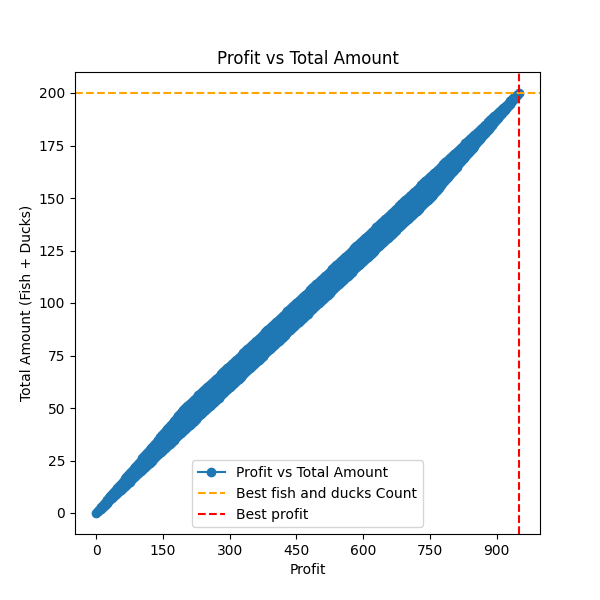
\includegraphics[width=0.5\textwidth]{figures/result_plot.png} 
  \caption{Replication result}
  \label{fig:yourlabel}
\end{figure}


\section{Conclusion}
To conclude, the main question to answer is: \textbf{\textit{Will I be able to get the same total profit and same count of ducks and fish to produce for December, using the same initial data, but tool from a different source?}}


%\clearpage

\bibliographystyle{ACM-Reference-Format}
\bibliography{sample}

\end{document}
\endinput
